\documentclass[11pt, a4paper]{article}
\usepackage[utf8x]{inputenc}
\usepackage[sort]{natbib}

\usepackage[spanish]{babel}
\usepackage{enumitem}
\usepackage{graphicx}
\usepackage{float}
\usepackage[linktoc=all]{hyperref}

\usepackage{etoolbox}

\usepackage{amsmath}
\usepackage{amssymb}
\usepackage{array}
\usepackage{gensymb}

\usepackage{fancyhdr}
\usepackage{multirow}
\usepackage{multicol}
\usepackage[table]{xcolor}
\usepackage{color}
\usepackage{colortbl}
\definecolor{lightgray}{gray}{0.9}
\setlength{\columnsep}{0.5cm}

\usepackage{tikz}
\usetikzlibrary{shapes.geometric, arrows}
\tikzstyle{problema} = [rectangle, rounded corners,  minimum width=3cm, minimum height=1cm,text centered, draw=black,fill={rgb:black,1;white,30}]
\tikzstyle{causa} = [rectangle, minimum width=3cm, minimum height=1cm, text centered, text width=4cm, draw=black, fill={rgb:black,0;white,10}]
\tikzstyle{nodo} = [diamond, minimum width=1cm, minimum height=1cm, text centered, draw=black, fill={rgb:black,0;white,10}]
\tikzstyle{arrow} = [thick,->,>=stealth]



%------------------- Dimensiones -------------------
\usepackage{geometry}
 \geometry{a4paper,total={170mm,257mm},left=15mm,right=15mm,top=20mm,}
%----------------------------------------------------

%------------------- Encabezado y Pie de pág -------------------
\pagestyle{fancy}
\fancyhf{}
\lhead{Electrónica de Potencia}
\rhead{TP7 : Llave H}
\rfoot{Página \thepage}
%----------------------------------------------------


%----------------------------- Documento -----------------------------------------------
\begin{document}
\begin{titlepage}
 \centering
	
\includegraphics[scale=0.80]{Imagenes/LOGO.jpg} \par
 	\vspace{1cm}
 	{\scshape\LARGE Universidad Tecnológica Nacional \par}
 	{\scshape\large Facultad Regional de Córdoba \par}
 	\vspace{1cm}
	{\bfseries \Large Trabajo Práctico De Laboratorio $N^{\circ} 7$\par}
	{\bfseries \Large Control de velocidad para motor de CC a lazo abierto\par}
 	\vspace{1.5cm}

	\begin{tabular}{ll}
		Alassia, Francisco		&	60861	\\
		Amaya, Matías			&	68284	\\
		Lamas, Matías			&	65536 	\\
		Navarro, Facundo		&	63809 	\\
		Veron, Misael			&	62628
	\end{tabular}
	
	\vspace{1cm}
	Curso: 5r2 \\
	Grupo $N^{\circ} 11$
 	\vfill
	{\bfseries \Large Electrónica de Potencia \par}

	\vspace{1.5cm}
	Docentes: \par
	Ing. Oros, Ramón \par
	Ing. Avramovich, Javier \par

 	\vfill
	{\large \today\par}
\end{titlepage}
	
	
\tableofcontents
\clearpage

%----------------your title below -----------------------------
\section{Introducción}

Se denomina Puente H al circuito electrónico que permite a un motor de continua girar en ambos sentidos. Su nombre se debe a la disposición de los interruptores, que se observa en el esquema de la Figura \ref{fig:puenteH}

\begin{figure}[h]
	\centering
	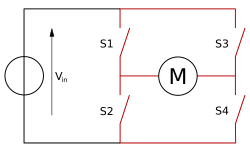
\includegraphics[width=6cm]{Imagenes/puenteH}
	\caption{Esquemático del Puente H.}
	\label{fig:puenteH}
\end{figure} 

El circuito funciona de la forma graficada en la Figura \ref{fig:puenteH_operacion}. Si consideramos el borne izquierdo del motor como el positivo, y el derecho como el negativo, cuando los interruptores S1 y S4 se cierran y S2 y S3 están abiertos, se aplica una tensión positiva en el motor, haciéndolo girar en un sentido. Invirtiendo esta configuración, es decir, abriendo los interruptores S1 y S4 y cerrando S2 y S3, el voltaje se invierte, logrando así que el motor gire en sentido inverso. 

Es importante remarcar que los interruptores de una misma rama no deben estar cerrados en un mismo instante de tiempo ya que ocasionarían un
corto circuito en la fuente de tensión. 

\begin{figure}[h]
	\centering
	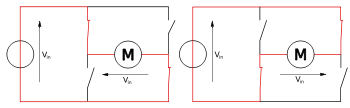
\includegraphics[width=13cm]{Imagenes/puenteH_operacion}
	\caption{Funcionamiento del Puente H.}
	\label{fig:puenteH_operacion}
\end{figure} 

Para lograr una modificación de la velocidad del motor -sin variar el par motriz- es necesario cambiar la tensión de alimentación del inducido sin modificar la corriente. Esto se logra con la modulación por ancho de pulso. 

La técnica de control mediante PWM se basa en la modificación del ciclo de trabajo de la señal que llega al controlador de los transistores que manejan la alimentación del motor, variando entre una conexión directa e inversa, donde la relación entre el ambos períodos determina el sentido y velocidad de giro del rotor.

Para lograr esto es necesario contar con 2 señales PWM complementarias que manejen una combinación de transistores cada una. En otras palabras, la suma de ambas señales debe significarle al motor un Dutty Cycle efectivo al motor lo mas cercano al 100\% posible, buscando así mantener el par motriz.


\section{Enunciado}
\begin{enumerate}
	\item Diseñar y construir un circuito que controle un motor de CC ( Ej. Mabuchi de 12V sin el regulador interno) en los cuatro cuadrantes con PWM y llave H con transistores MOSFET IRF830 con protección contra sobrecorrientes en el driver de compuerta, o en la llave H.
	
	El circuito será a lazo abierto. Tensión de referencia: +/- 5V (puede ser otro valor).
	
	Frecuencia de conmutación: 15khz, y contador de revoluciones con MOC70U1 (o equivalente)

	\item Efectuar las siguientes mediciones:
	\begin{enumerate}
		\item Graficar las RPM del motor en función de la tensión de referencia.
		\item Verificar funcionamiento del sist. de protección contra sobrecorrientes
	\end{enumerate}
\end{enumerate}

\section{Circuito}
\subsection{Actuador}


\begin{figure}[h]
	\centering
	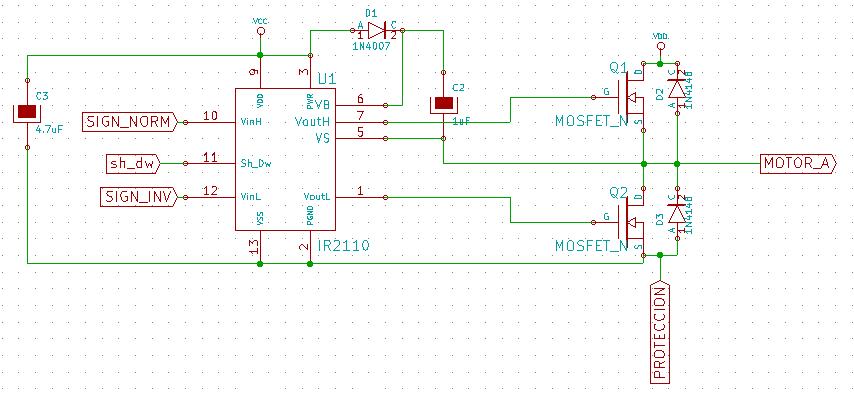
\includegraphics[width=\textwidth]{Imagenes/circ_driver.png}
	\caption{Medio puente H.}
	\label{fig:circ_driver}
\end{figure} 

El puente H está formado por 2 bloques simétricos, compuestos por dos transistores cada uno, controlados por un driver. Este circuito se puede observar en la Figura \ref{fig:circ_driver}.

\subsubsection{Transistores}

Para la realización del puente se utilizaron transistores MOSFET del tipo N modelo IRF840, como se solicita en la consigna. Estos transistores poseen un diodo conectado en paralelo que permiten a las corrientes circular en sentido inverso al previsto, situación que se da en la conmutación debido a las propiedades inductivas del bobinado del motor.

\subsubsection{Driver}
Para el control de los transistores se emplearon IR2110. Estos drivers poseen la particularidad de entregar dos salidas denominadas \textit{High Output} y \textit{Low Output}, de referencia independiente, lo que permite manejar ambos transistores de una rama con el mismo integrado.

Este bloque posee 3 entradas. Por un lado, las entradas \textit{NO\_INV} y \textit{INV} serán las señales complementarias de PWM que exitarán al transistor superior e inferior respectivamente. Es necesario aclarar que en cada uno de los dos bloques \textit{"Puente H"} que componen el circuito, estas dos señales deben estar intercambiadas de posición para lograr el patrón de encendido y apagado de los transistores correctamente.

Adicionalmente a las dos señales de control, se encuentra la señal \textit{SD} o Shutdown que permite inhabilitar el driver. Esta señal la utilizaremos mas adelante en el bloque de protección (Sec. \ref{sec:proteccion}) para deshabilitar los motores ante una \textit{sobrecorriente}.

\vfill
\subsection{Control}
\subsubsection{Generador de PWM}
La etapa de generación de $PWM$, posee la función de generar el pulso de ancho variable, que será finalmente
el encargado de regular tanto la velocidad como el sentido de giro del motor.

Para este bloque utilizamos el integrado TL494. La principal característica de este integrado es la posibilidad de variar el ancho de pulso hasta un Dutty Cycle del 97\%. Para este caso, se calcularon los componentes para una frecuencia de trabajo de 15$kHz$.

Para la implementación utilizamos un preset para la regulación de la frecuencia, en la pata 6 del integrado, y un potenciómetro para la variación del ciclo de trabajo conectado al feedback (pin 3).

La frecuencia de trabajo está dada por la constante de tiempo de los capacitores en las patas 5 y 6. 

\begin{equation}
f_{osc} = \frac{1}{R_T \cdot C_T} 
\end{equation}

Eligiendo un capacitor de $10 \; nF$
\begin{equation}
	f_{osc} = \frac{1}{R_T \cdot C_T} \; \therefore \; R_T = \frac{1}{f_{osc} \cdot C_T} = \frac{1}{15 \; kHz \cdot 10 \; nF} = 6667 \; \Omega 
\end{equation}

Para esto se coloca una resistencia de $2.2 \; k\Omega$ en serie con una resistencia variable ($RV4$) para regular la frecuencia hasta alcanzar el valor esperado.

El circuito que regula el ciclo de trabajo se varía con un potenciómetro lineal de $1 \; k\Omega$ y los límites de tensión que acepta la entrada de control de ciclo de trabajo, tanto el inferior como el superior, se controlaron de forma práctica mediante trimmers ajustables linealizando el potenciómetro $RV2$ logrando una excursión completa.

\begin{figure}[h]
	\centering
	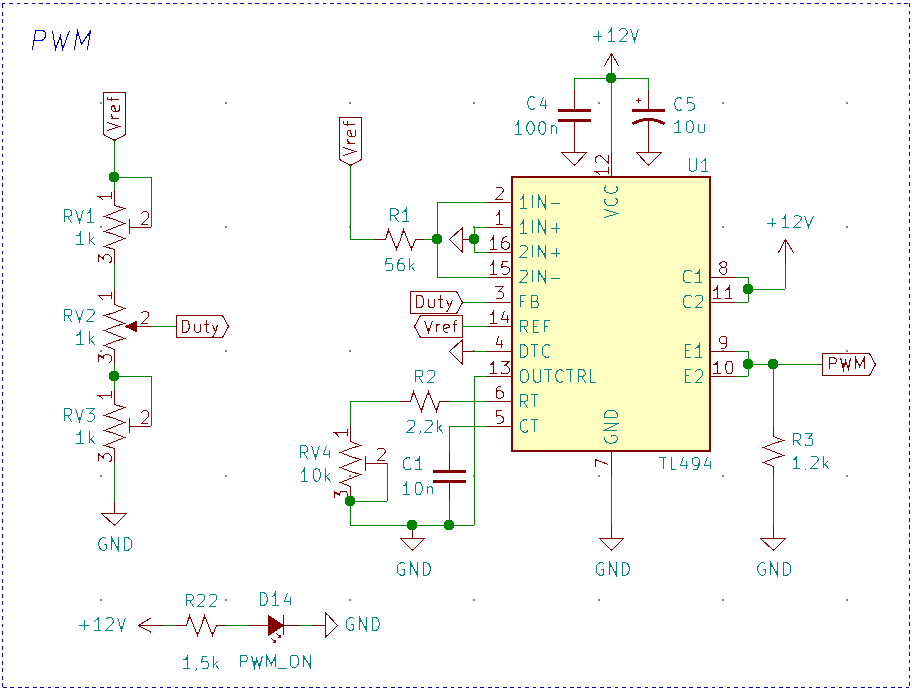
\includegraphics[width=0.8\textwidth]{Imagenes/circ_pwm.png}
	\caption{Generador de PWM}
	\label{fig:circ_pwm}
\end{figure} 


 \subsubsection{Generador de Tiempos Muertos}

El circuito generador de tiempos muertos ilustrado en la Figura \ref{fig:circ_retardo} es el encargado de generar un defasaje entre las señales de control, necesario para evitar que los dos transistores de la misma rama se exciten al mismo tiempo. 


El funcionamiento del circuito es el de un retardador con compuertas negadoras analizado en Técnicas Digitales I. Cuando en la entrada PWM hay un 0 lógico, a la salida de la primer compuerta obtenemos un 1 que cargará el capacitor rápidamente a través del diodo, lo que podrá un 1 en la entrada de la segunda compuerta y un 0 a la salida de la rama. Luego, cuando a la entrada hay un 1, en la salida del primer inversor habrá un 0 que descargará el capacitor luego de un tiempo dado por el ajuste de la resistencia y el capacitor, esto hará que la segunda compuerta demore en detectar el 0 retardando la aparición del 1 lógico a su salida.

La rama inferior incorpora una compuerta inversora extra, lo que invierte la señal produciendo la señal complementaria.

\begin{figure}[h]
	\centering
	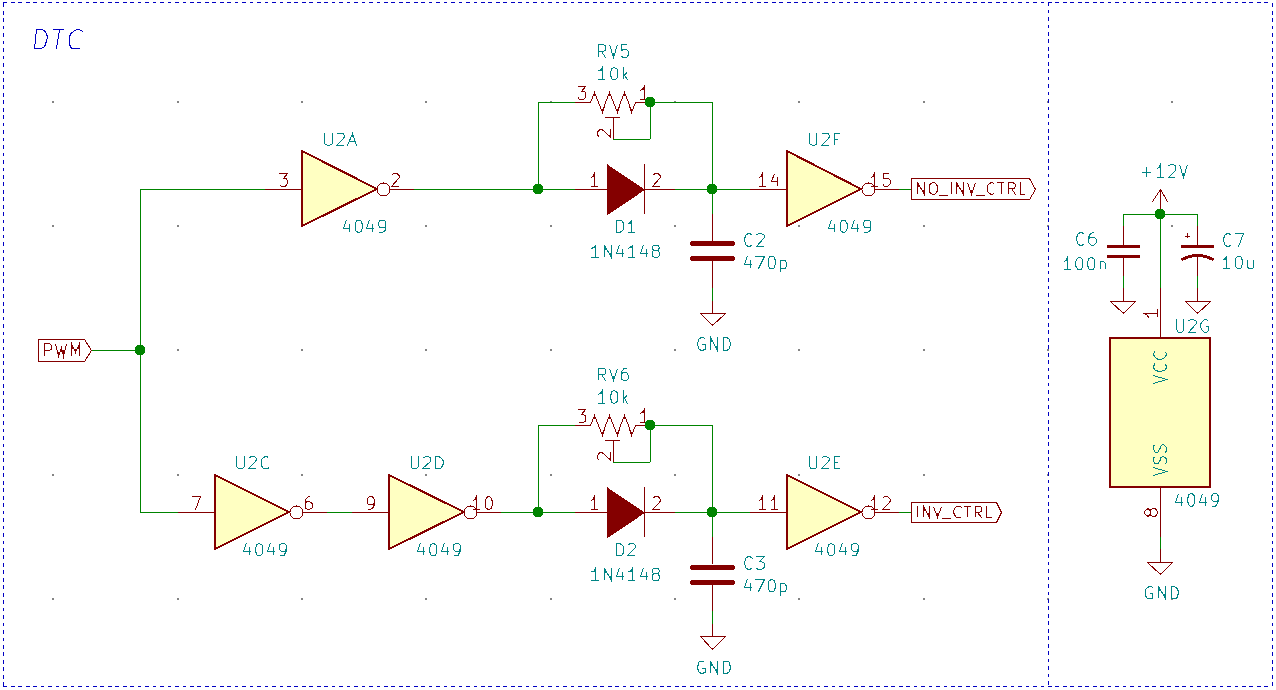
\includegraphics[width=0.9\textwidth]{Imagenes/circ_retardo.png}
	\caption{Circuito de Retardo}
	\label{fig:circ_retardo}
\end{figure} 

Este tiempo muerto es necesario ya que los transistores poseen un tiempo entre el momento en el que la señal de control vuelve a 0 y el momento en el que se apagan. Este retardo se ilustra en la hoja de datos del transistor como \textit{Turn-Off Delay Time} $t_{off}$. Para garantizar una operación segura, exageramos este tiempo entre pulso y pulso a 2 [µs], debido a que las condiciones de funcionamiento no son iguales a las de utilizadas en las pruebas que realiza el fabricante, ni los transistores fabricados poseen exactas características entre sí. Las demoras de cada salida serán las de propagación de la compuerta, más la del circuito de tiempo. 


\begin{equation}
\tau = 0.693 \cdot R \cdot C
\end{equation}

\begin{equation}
2 \; us = R \cdot 470 \; pF
\end{equation}

\begin{equation}
R = \frac{2 \; us }{470 \; pF} = 4255 \Omega
\end{equation}

En adición a la constante de tiempo utilizada para generar el retardo, se suma los retardos de propagación de las compuertas negadoras, que en el caso del CD4049 es de $30nS$ c/u para $5V$.

Para controlar el tiempo de delay se utilizan trimmers como la resistencia calculada del circuito de retardo.

\subsection{Protección}\label{sec:proteccion}
De las especificaciones de diseño es necesario implementar un circuito detector y protector contra sobrecorrientes en el motor. Este circuito presenta una elevada utilidad, sobre todo si se trata de un motor de gran potencia, ya que si por alguna falla o desperfecto el rotor se llegase a bloquear, la corriente que circularía a bornes del mismo aumentaría drásticamente como consecuencia de un aumento desmesurado en el par de carga. Esto conlleva al mismo aumento en la corriente circulante por el “driver” del motor y podría provocar la destrucción del circuito.

Para proteger el circuito de sobre corrientes, incluimos el bloque de protección detallado en la Figura \ref{fig:circ_protecc}.

A la salida del puente H, en serie con el motor, colocamos una resistencia sensora con el objetivo de medir la corriente que circula por el motor. Esta tensión medida, equivalente a la corriente, es comparada con una referencia fijada por un potenciómetro. A la salida del comparador, la señal resultante activa el pin de Shutdown \textit{SD} de los drivers.

Consecuentemente el motor se detendrá. Como último, para devolver el funcionamiento al motor, se reinicia al flip−flop D mediante un reset manual.

Para calibrar la protección se coloca el motor a girar a las revoluciones deseadas y se calibra para que, al aplicar fuerza extra sobre el eje, la protección se active. Esto garantiza un margen de corriente en el que el funcionamiento sea normal y que al aumentar la corriente, por un esfuerzo extra, la protección se active.


\begin{figure}[h]
	\centering
	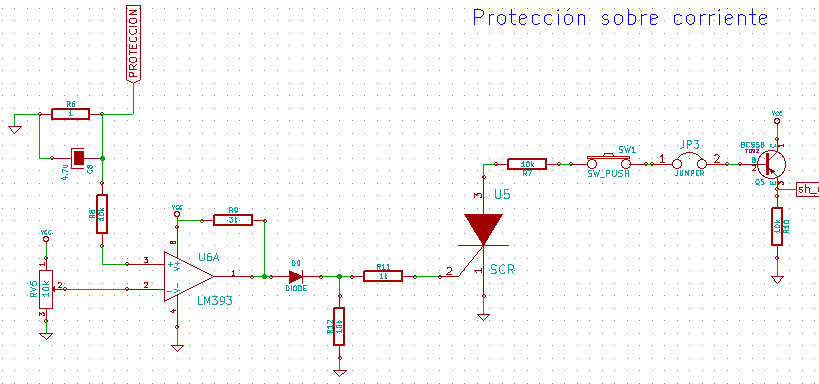
\includegraphics[width=\textwidth]{Imagenes/circ_prot.png}
	\caption{Circuito de Protección}
	\label{fig:circ_protecc}
\end{figure} 

El circuito comparador que se utilizó es el $LM393$. Sus características son:
\begin{itemize}
	\item High precision comparators (es un comparador de precisión, diseñado con este fin).
	\item Corriente de polarización de entrada: $25\; nA$.
	\item Tensión de offset máxima: $\pm 3 \; mV$.
    \item Baja corriente de offset en la entrada $\pm 5 \; nA$.
\end{itemize}

Este circuito integrado, a diferencia de cualquier otro amplificador operacional (aunque existen varios con características similares), son comparadores de precisión, diseñados para este único fin. Particularmente como en este caso se necesita comparar tensiones de bajo valor (pues es un proceso de censado), entonces mientras mejores características posea este comparador mejor para la aplicación, ya que de este modo se evita determinados conflictos como el enmascaramiento de la señal a medir con ruido, o la oscilación por el ruido del motor.

Como último detalle, este operacional es diseñado a colector abierto (“Open Colector”), por lo que necesita para
su funcionamiento una resistencia de pull-up de $1 \; k\Omega$ según especificaciones del fabricante.

\clearpage

\section{Mediciones}

En la Figura \ref{fig:osc_max} se observa el PWM obtenido para la condición de máxima velocidad del motor. En ella se puede apreciar los tiempos muertos entre ambas señales y el concepto del toque constante. 

Por otro lado, en la Figura \ref{fig:osc_min} ambas señales poseen un dutty cycle del 50\%, lo que provoca que el motor se detenga pero mantenga el torque.

\begin{figure}[h!]
	\centering
	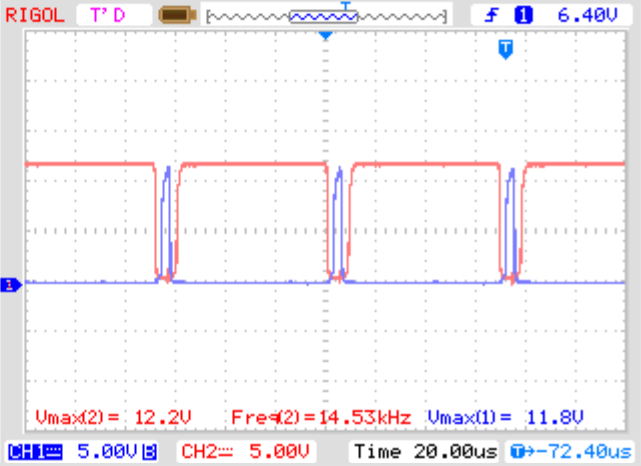
\includegraphics[width=0.7\textwidth]{Imagenes/osc_max.png}
	\caption{PWM para motor a máxima velocidad}
	\label{fig:osc_max}
\end{figure} 

\begin{figure}[h!]
	\centering
	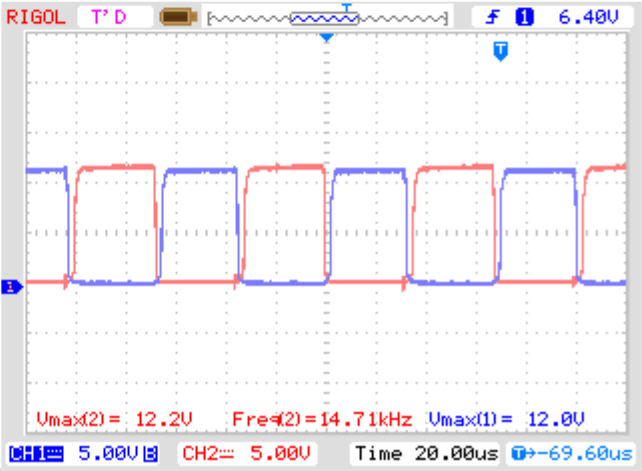
\includegraphics[width=0.7\textwidth]{Imagenes/osc_min.png}
	\caption{PWM para detención del motor}
	\label{fig:osc_min}
\end{figure} 

\subsection{Volts vs RPM}
El circuito planteado para la medición de las revoluciones se observa en la Figura \ref{fig:circ_rpm}, el mismo consiste en el sensor $TCST1103$, el cual esta formado por un emisor infrarrojo y un fototransistor ubicado frente a frente en un encapsulado en forma de horquilla, se construye un soporte para el motor y colocando sobre el eje una rueda con perforaciones que funciona a modo de encoder, como se ve en la figura \ref{fig:pcb_rpm}. Para asegurar que a la salida se vea una onda cuadrada se usa un comparador $LM393$ que tal como se explico previamente funciona comparando sus entradas, haciendo que el valor analógico provisto por el sensor sea digitalizado a su salida. 
\begin{figure}[h!]
	\centering
	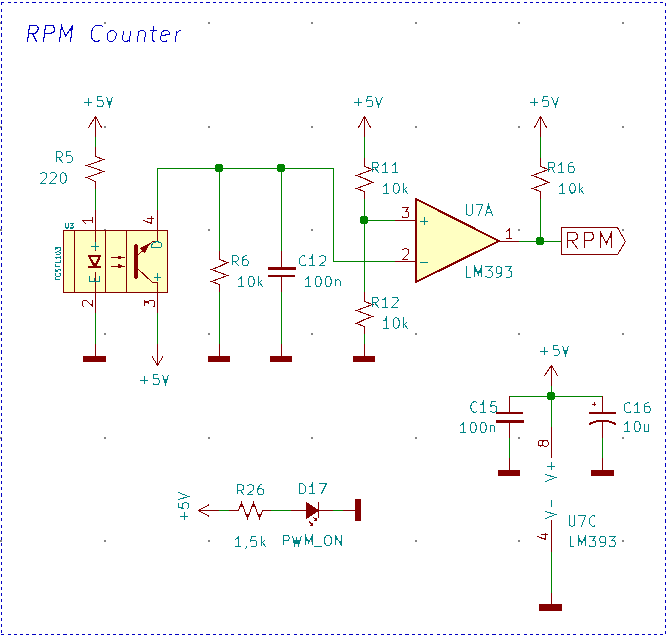
\includegraphics[width=0.6\textwidth]{Imagenes/circ_rpm.png}
	\caption{Circuito para medir RPM}
	\label{fig:circ_rpm}
\end{figure} 

\begin{figure}[h!]
	\centering
	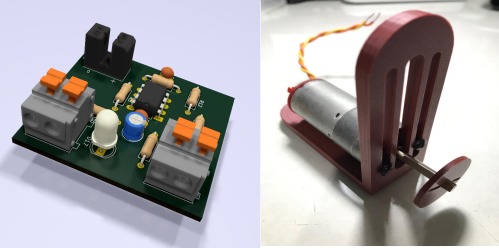
\includegraphics[width=0.9\textwidth]{Imagenes/rpm_pcb.png}
	\caption{PCB para circuito RPM}
	\label{fig:pcb_rpm}
\end{figure} 


Una vez obtenida la frecuencia de giro del motor, mediante el circuito  anterior, se determinan las RPM,a través de la siguiente ecuación:

\begin{equation}
	RPM = \frac{f_{medida} \cdot 60}{N}
\end{equation}

donde

\begin{itemize}
	\item $f_{medida}$ = es la frecuencia obtenida en el osciloscopio, por medio del circuito previamente expuesto.
	\item $60$ = es la constante por la cual multiplicamos la frecuencia, de modo tal que el factor temporal sea $1 \; minuto$ 
	\item $N$ = es la cantidad de veces en un giro que se corta el haz del emisor infrarrojo. Mientras mayor sea mayor sera la frecuencia obtenida y por ende para no afectar la medición debe dividirse por esta cantidad.
\end{itemize}

Los resultados se exponen a continuación

\begin{figure}[h]
	\centering
	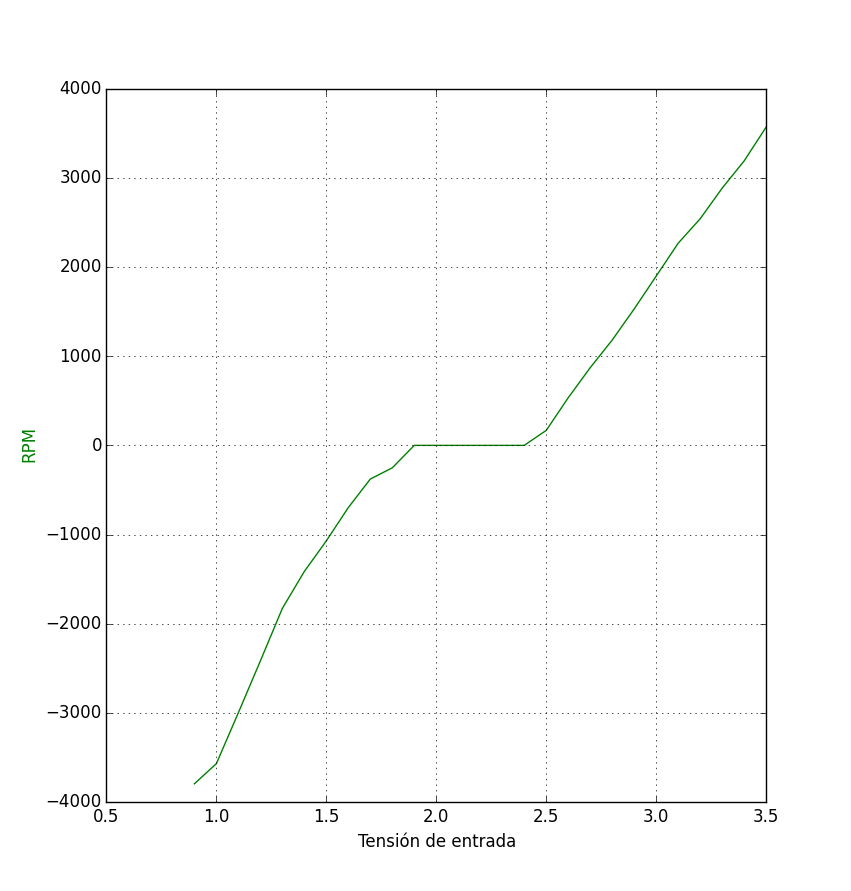
\includegraphics[width=15cm]{Imagenes/rpm.png}
	\caption{Curva de Tensión vs RPM}
	\label{fig:rpm}
\end{figure} 

  
\subsection{Protección}
Se ajustó la tensión de referencia en un valor tal que al forzar el motor, el circuito actuara y lo detuviera. La protección funcionó tal y como se esperaba, deteniendo la marcha hasta el momento en el que se presionó el pulsador de liberación.


\section{Conclusiones}
La implementación del circuito conllevó una dificultad mínima, logrando muy buenos resultados. El puente H resulta muy útil para controlar no solo la velocidad de giro, si no también el sentido de giro y lograr una frenada instantánea.

En este práctico, la señal de PWM la obtuvimos de un circuito integrado, controlando la velocidad mediante una señal de referencia, pero este circuito podría ser reemplazado por un microcontrolador y controlar la velocidad del motor digitalmente.

El circuito ha demostrado ser eficaz para el control de la velocidad y sentido de giro de motores de corriente continua de baja potencia, otorgando una curva de comando de dichas características de notable simetría. Si bien su característica de control es prácticamente manual, dado que el ancho de la señal pulsante así como la posibilidad de reinicio son únicamente controlables por el usuario para este circuito, la morfología del diseño empleado otorga versatilidad y facilidades para adaptarlo e incluirlo en un sistema de control automatizado o de mayor precisión.
Respecto al sistema de control de la velocidad y sentido de giro con la variación del cursor del  potenciómetro se observa de la curva completa de funcionamiento un pequeño entorno de no movimiento distribuido alrededor del valor de ciclo de trabajo de 50\% que es donde el motor no dispone del par suficiente para vencer su inercia. Se ha logrado reducir dicho entorno al calibrar los resistores ajustables en la misma rama del potenciómetro, de modo de lograr una aparente linealidad en todo el rango.

El modelo de control indicado por la topología utilizada es de cuatro cuadrantes, donde en el primero y tercero funciona como motor con sentido de giro contrario para cada caso, y en el segundo y cuarto cuadrante el motor actúa frenando el rotor. Evidentemente la acción de freno está instintivamente asociada cuando de los extremos de máxima velocidad se tiene a un ciclo de trabajo del 50\%. Básicamente, la disminución de velocidad se debe a la disminución de la tensión del inducido porque la tensión promedio diferencial aplicada a cada diagonal tiende a cero.

\end{document}
